% Gerado por scripts/gerar-figuras-monografia.py; não editar.
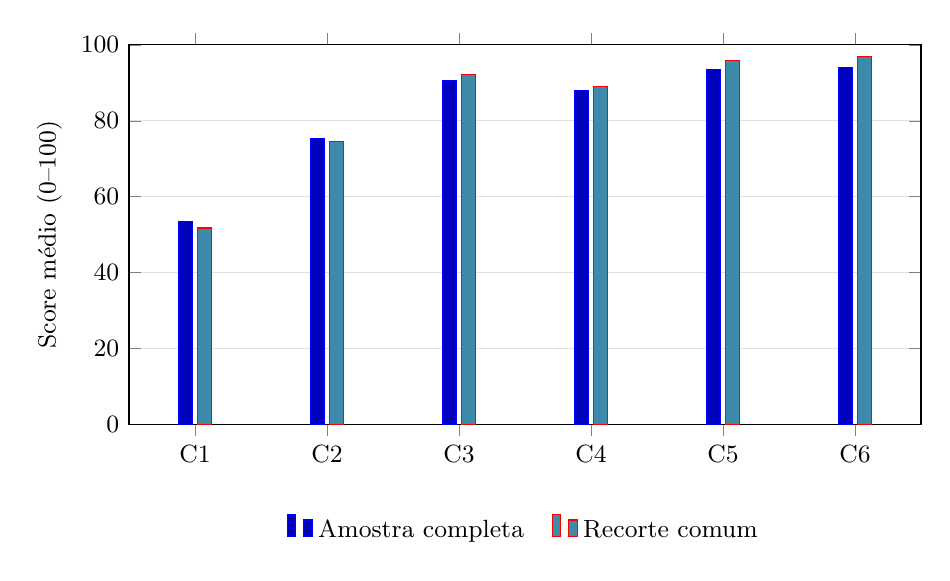
\begin{tikzpicture}
\begin{axis}[
width=0.96\textwidth,height=6.4cm,
tick label style={font=\small},label style={font=\small},
legend style={font=\small,at={(0.5,-0.22)},anchor=north,legend columns=3,draw=none,/tikz/every even column/.append style={column sep=8pt}},
ymajorgrids=true,grid style={black!12},
ybar,bar width=5pt,ymin=0,ymax=100,ylabel={Score médio (0--100)},xtick={1,2,3,4,5,6},xticklabels={C1,C2,C3,C4,C5,C6},enlarge x limits=0.1,legend columns=2
]
\addplot+[ybar,fill=blue!75!black] coordinates {(1,53.37500000) (2,75.22500000) (3,90.62500000) (4,87.87500000) (5,93.50000000) (6,94.12500000)};
\addlegendentry{Amostra completa}
\addplot+[ybar,fill=cyan!65!black] coordinates {(1,51.75000000) (2,74.62500000) (3,92.18750000) (4,89.06250000) (5,95.93750000) (6,96.87500000)};
\addlegendentry{Recorte comum}
\end{axis}
\end{tikzpicture}
